\documentclass{standalone}
\usepackage{tikz}
\usepackage{amsmath}

\begin{document}

\tikzset{every picture/.style={line width=0.75pt}} %set default line width to 0.75pt

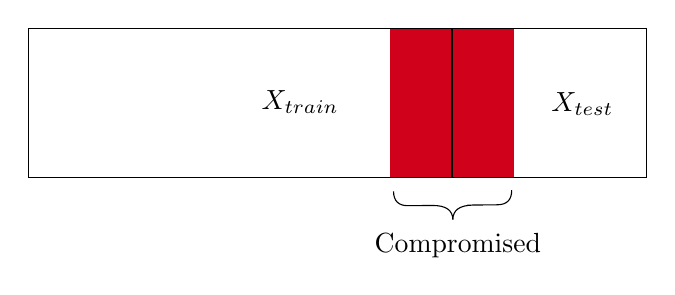
\begin{tikzpicture}[x=0.75pt,y=0.75pt,yscale=-1,xscale=1]
%uncomment if require: \path (0,122.01666259765625); %set diagram left start at 0, and has height of 122.01666259765625

%Shape: Rectangle [id:dp9410226493558759]
\draw   (180,1.43) -- (477.92,1.43) -- (477.92,73.43) -- (180,73.43) -- cycle ;
%Shape: Rectangle [id:dp275820482327108]
\draw  [draw opacity=0][fill={rgb, 255:red, 208; green, 2; blue, 27 }  ,fill opacity=1 ] (354.08,1.96) -- (384,1.96) -- (384,73.16) -- (354.08,73.16) -- cycle ;
%Shape: Rectangle [id:dp6212831419718663]
\draw  [draw opacity=0][fill={rgb, 255:red, 208; green, 2; blue, 27 }  ,fill opacity=1 ] (384,1.96) -- (413.92,1.96) -- (413.92,73.16) -- (384,73.16) -- cycle ;
%Straight Lines [id:da8449023188819424]
\draw [line width=0.75]    (384,1.96) -- (384,73.16) ;


%Shape: Brace [id:dp2396193508788067]
\draw   (356,80) .. controls (356.05,84.67) and (358.4,86.98) .. (363.07,86.93) -- (374.53,86.82) .. controls (381.2,86.75) and (384.55,89.05) .. (384.6,93.72) .. controls (384.55,89.05) and (387.86,86.69) .. (394.53,86.62)(391.53,86.65) -- (405.99,86.5) .. controls (410.66,86.45) and (412.97,84.1) .. (412.92,79.43) ;

% Text Node
\draw (311,37) node   {$X_{train}$};
% Text Node
\draw (447,38) node   {$X_{test}$};
% Text Node
\draw (387,106) node  [align=left] {Compromised};


\end{tikzpicture}

\end{document}
